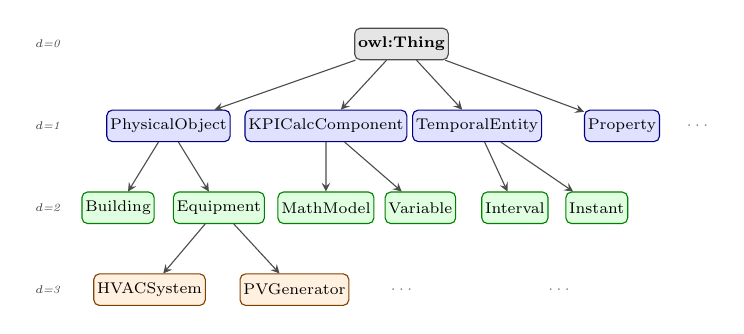
\begin{tikzpicture}[
    scale=0.8, transform shape,
    every node/.style={font=\scriptsize},
    class/.style={rectangle, rounded corners=2pt, draw, minimum height=5mm, align=center, inner sep=1.5pt},
    root/.style={class, fill=gray!20, draw=gray!60!black, font=\scriptsize\bfseries},
    level1/.style={class, fill=blue!12, draw=blue!50!black},
    level2/.style={class, fill=green!12, draw=green!50!black},
    level3/.style={class, fill=orange!12, draw=orange!50!black},
    edge/.style={draw, ->, >=stealth, gray!60!black},
    depthlabel/.style={font=\tiny\itshape, text=gray!50!black}
]

% Depth labels on the left (moved further left)
\node[depthlabel, anchor=east] at (-0.8, 0) {$d$=0};
\node[depthlabel, anchor=east] at (-0.8, -1.3) {$d$=1};
\node[depthlabel, anchor=east] at (-0.8, -2.6) {$d$=2};
\node[depthlabel, anchor=east] at (-0.8, -3.9) {$d$=3};

% Level 0: Root
\node[root] (thing) at (4.5, 0) {owl:Thing};

% Level 1: Top-level categories (from BEO ontology)
\node[level1] (physical) at (0.8, -1.3) {PhysicalObject};
\node[level1] (kpicomp) at (3.3, -1.3) {KPICalcComponent};
\node[level1] (temporal) at (5.7, -1.3) {TemporalEntity};
\node[level1] (property) at (8, -1.3) {Property};

% Level 2: Sub-categories
\node[level2] (building) at (0, -2.6) {Building};
\node[level2] (equipment) at (1.6, -2.6) {Equipment};
\node[level2] (mathmodel) at (3.3, -2.6) {MathModel};
\node[level2] (variable) at (4.8, -2.6) {Variable};
\node[level2] (interval) at (6.3, -2.6) {Interval};
\node[level2] (instant) at (7.6, -2.6) {Instant};

% Level 3: Leaf classes (moved apart to avoid overlap)
\node[level3] (hvac) at (0.5, -3.9) {HVACSystem};
\node[level3] (pv) at (2.8, -3.9) {PVGenerator};

% Edges from root
\draw[edge] (thing) -- (physical);
\draw[edge] (thing) -- (kpicomp);
\draw[edge] (thing) -- (temporal);
\draw[edge] (thing) -- (property);

% Edges from Level 1
\draw[edge] (physical) -- (building);
\draw[edge] (physical) -- (equipment);
\draw[edge] (kpicomp) -- (mathmodel);
\draw[edge] (kpicomp) -- (variable);
\draw[edge] (temporal) -- (interval);
\draw[edge] (temporal) -- (instant);

% Edges from Level 2
\draw[edge] (equipment) -- (hvac);
\draw[edge] (equipment) -- (pv);

% Ellipsis nodes to indicate more classes
\node[font=\scriptsize, text=gray] at (4.5, -3.9) {$\cdots$};
\node[font=\scriptsize, text=gray] at (7, -3.9) {$\cdots$};
\node[font=\scriptsize, text=gray] at (9.2, -1.3) {$\cdots$};

\end{tikzpicture}
